%% ****** Start of file apstemplate.tex ****** %
%%
%%
%%   This file is part of the APS files in the REVTeX 4 distribution.
%%   Version 4.1r of REVTeX, August 2010
%%
%%
%%   Copyright (c) 2001, 2009, 2010 The American Physical Society.
%%
%%   See the REVTeX 4 README file for restrictions and more information.
%%
%
% This is a template for producing manuscripts for use with REVTEX 4.0
% Copy this file to another name and then work on that file.
% That way, you always have this original template file to use.
%
% Group addresses by affiliation; use superscriptaddress for long
% author lists, or if there are many overlapping affiliations.
% For Phys. Rev. appearance, change preprint to twocolumn.
% Choose pra, prb, prc, prd, pre, prl, prstab, prstper, or rmp for journal
%  Add 'draft' option to mark overfull boxes with black boxes
%  Add 'showpacs' option to make PACS codes appear
%  Add 'showkeys' option to make keywords appear
\documentclass[aps,prb,twocolumn,superscriptaddress]{revtex4-1}
\usepackage{natbib}
\usepackage{graphicx,amssymb,amsmath,ifthen}
\usepackage{bm}
\usepackage{braket}
\newcommand{\angstrom}{\mbox{\normalfont\AA}}

%\documentclass[aps,prl,preprint,superscriptaddress]{revtex4-1}
%\documentclass[aps,prl,reprint,groupedaddress]{revtex4-1}

% You should use BibTeX and apsrev.bst for references
% Choosing a journal automatically selects the correct APS
% BibTeX style file (bst file), so only uncomment the line
% below if necessary.
%\bibliographystyle{apsrev4-1}

\begin{document}

% Use the \preprint command to place your local institutional report
% number in the upper righthand corner of the title page in preprint mode.
% Multiple \preprint commands are allowed.
% Use the 'preprintnumbers' class option to override journal defaults
% to display numbers if necessary
%\preprint{}

%Title of paper
\title{Introduction to the Paul Trap and its Applications in Quantum Computing}

% repeat the \author .. \affiliation  etc. as needed
% \email, \thanks, \homepage, \altaffiliation all apply to the current
% author. Explanatory text should go in the []'s, actual e-mail
% address or url should go in the {}'s for \email and \homepage.
% Please use the appropriate macro foreach each type of information

% \affiliation command applies to all authors since the last
% \affiliation command. The \affiliation command should follow the
% other information
% \affiliation can be followed by \email, \homepage, \thanks as well.
\author{Christopher Moore}
\affiliation{Department of Physics and Astronomy, Clemson University, Clemson, SC 29634, USA}



%\email[]{Your e-mail address}
%\homepage[]{Your web page}
%\thanks{}
%\altaffiliation{}


%Collaboration name if desired (requires use of superscriptaddress
%option in \documentclass). \noaffiliation is required (may also be
%used with the \author command).
%\collaboration can be followed by \email, \homepage, \thanks as well.
%\collaboration{}
%\noaffiliation

\date{\today}

\begin{abstract}
Here we give a brief review of Paul traps. We begin with a historical context along with the experimental background. Next we use classical electrodynamics to give a rigorous proof detailing how the solutions to Laplace's equation yield ions which behave as simple harmonic oscillators which are "trapped" at the center of the potential for a broad range of energies. Finally we touch on one of the more interesting applications for Paul traps, trapped ion quantum computers.
\end{abstract}

% insert suggested PACS numbers in braces on next line
\pacs{}
% insert suggested keywords - APS authors don't need to do this
%\keywords{}

%\maketitle must follow title, authors, abstract, \pacs, and \keywords
\maketitle


Linear ion traps also known as Paul traps, invented by Wolfgang Paul in 1989 are a means of trapping ions using rotating electric fields.  When used in conjunction with laser cooling these traps give scientists a means to study quantum effects on the macroscopic level. These and other similar traps have also lead to practical applications such as quantum computing. In this paper we first explain the experimental set up and theory behind these traps.  Next we show how laser cooling has fueled a boom in experimental research into trapped ion quantum computing and finally we discuss a few modern experiments looking at this as a feasible step toward achieving a real quantum computer.
%%%%%%%%%%%%%%%%%%%%%%%%%%%%%%%%

An ion trap is a device which uses magnetic and electric fields to confine atoms. The goal of these traps is to isolate the ions from their environment, with scientific application such as spectroscopy and  quantum computing. For a particle to be confined the applied electric and magnetic potentials must form a stable equilibrium point such that small perturbations to the system in any direction will result in the ion "falling back" to its stable equilibrium point (Fig. \ref{fig:pot}). Thus the particle should be located within a potential minimum. Another way to state this is that all forces should push back toward the equilibrium point or that the divergence of the field lines should be negative creating a sink point.
Earnshaw's theorem states that is not possible to create such a stable stationary equilibrium using electrostatic interactions alone. This can be seen, by directly looking at Maxwell's equations for the electric and magnetic field lines in free space.
\begin{eqnarray}
\nabla\cdot E &=& 0\\
\nabla\cdot B &=& 0
\label{chiB}
\end{eqnarray}
It is clear that in the absence of point charges that there can be no stable equilibrium point and hence no way to trap ions using electrostatic forces alone. While there are no stable minima there are saddle points created (SEE FIG). A Paul trap is a trap which uses a series of parallel electrodes (usually 4) (SEE FIG) to create an electric field which traps ions using these saddle points. Each pair of rods is connected to the rod directly opposite from it such that the two rods have the exact same voltage. An alternating current is then applied between the two rods such that the pairs of rods are directly out of phase with one another. Creating the potentials,
\begin{equation}
\phi = \phi_0\pm\frac{V_0}{2}\cos{\Omega t}\\
\label{eq:pot}
\end{equation}
%%%%%%%%%%%%%%%%%%%%%%%%%%%%
\begin{figure}
	\begin{center}
		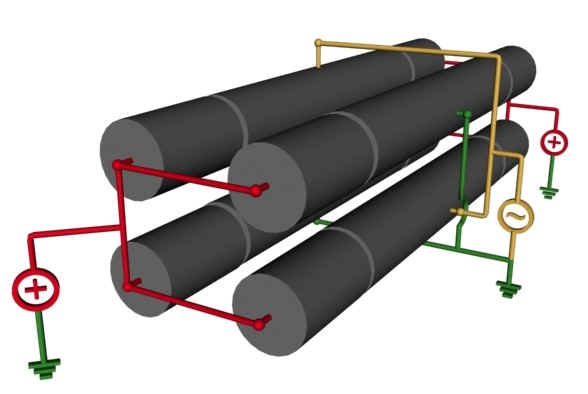
\includegraphics[width=0.48\textwidth]{expSetup}
	\end{center}
	\vspace{-2mm}
	\caption{Experimental schematic of a Paul Trap. Four parallel electrodes are set up with equal potentials applied to opposite electrodes.  The pairs of electrodes are then connected via alternating current on the order of microwave frequency.  this creates a rotating saddle point potential which will force ions to behave as quantum oscillators confining them within the counter of the trap.}
	\label{fig:setup}
	\vspace{-3mm}
\end{figure}
%%%%%%%%%%%%%%%%%%%%%%	
%%%%%%%%%%%%%%%%%%%%%%%%%%%%%%%%
with the first term representing the applied d.c. current and the second term the a.c. current. The alternating current creates the effect of rapidly rotating the electric field confining the particle within the saddle point of the potential, much like the mechanical analog shown in (FIG \ref{fig:mech}).
In order to show that this method will truly confine the particle within the trap we solve Laplace's equation
%%%%%%%%%%%%%%%%%%%%%%%%%%%%%%%%
%%%%%%%%%%%%%%%%%%%%%%%%%%%%
\begin{figure}
	\begin{center}
		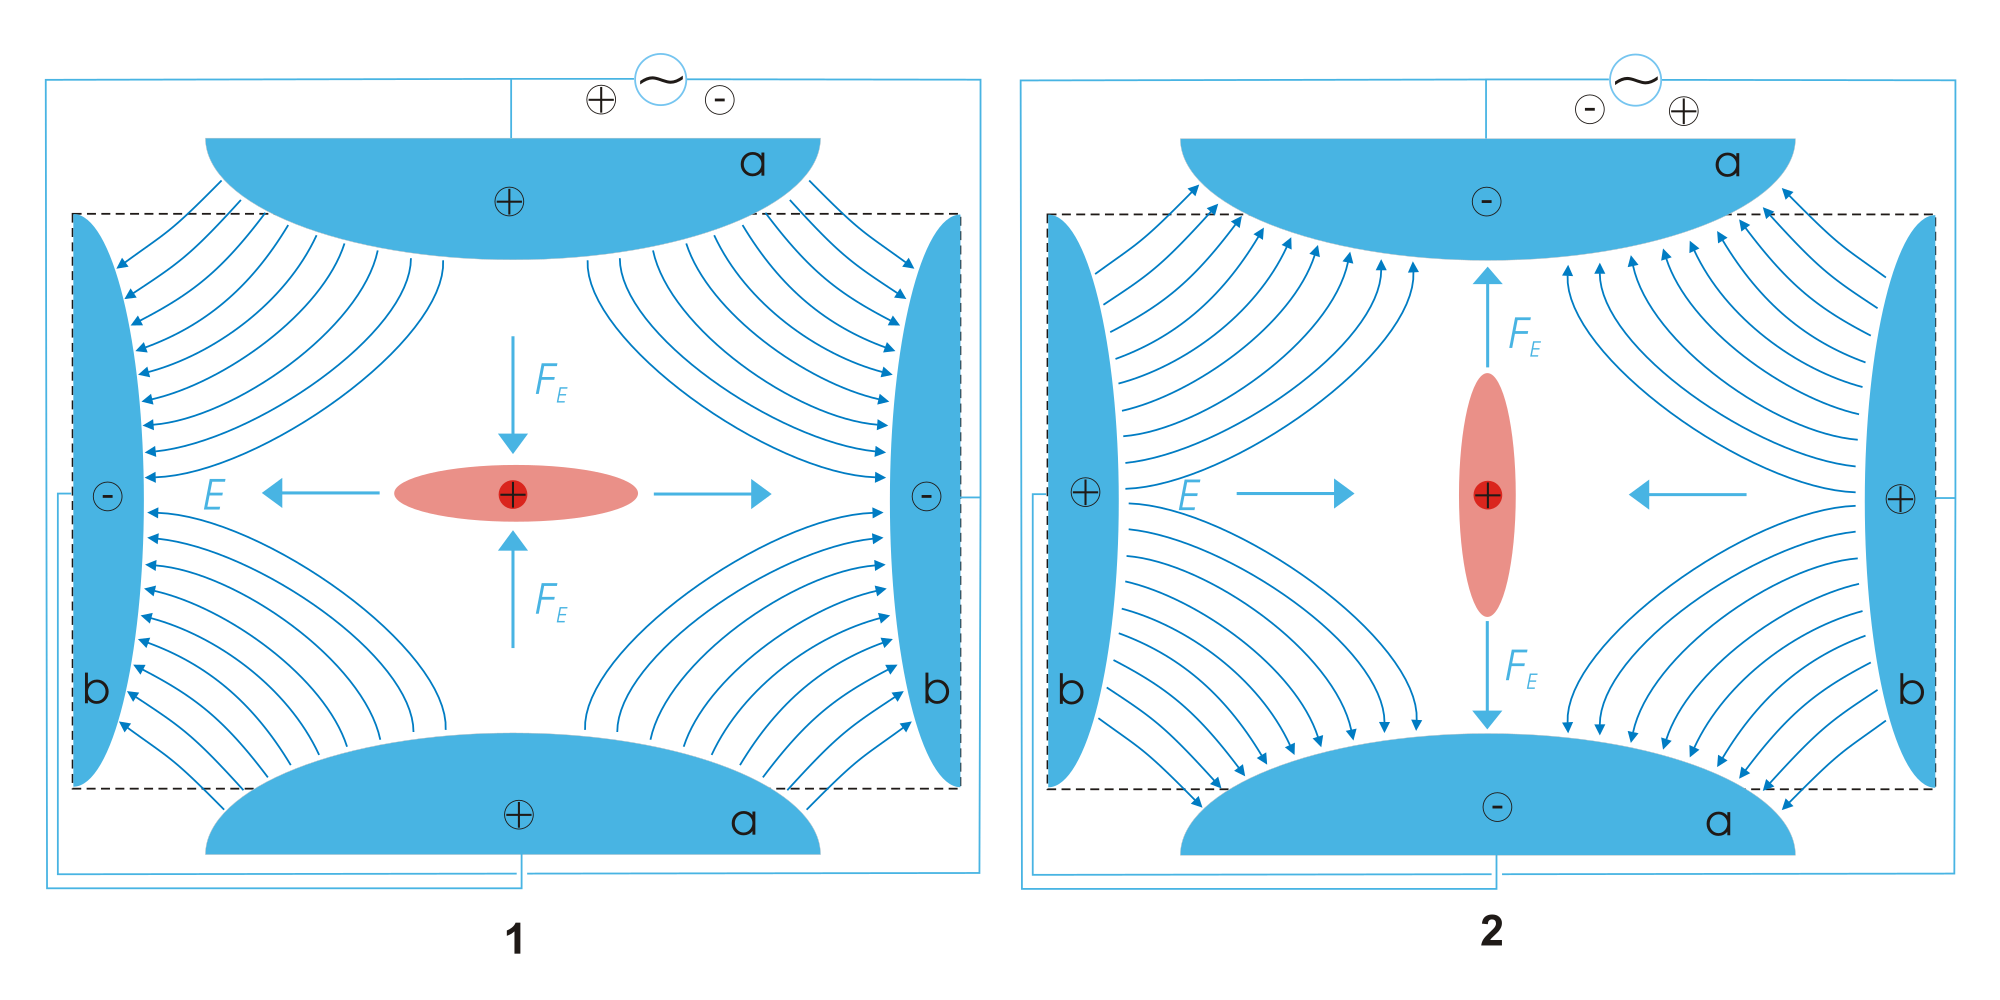
\includegraphics[width=0.48\textwidth]{2000px-Paul-Trap.png}
	\end{center}
	\vspace{-2mm}
	\caption{Electric fields created by Paul trap. Hyperbolic electrodes of opposite potential create a saddle point at the center of the trap.}
	\label{fig:pot}
	\vspace{-3mm}
\end{figure}
%%%%%%%%%%%%%%%%%%%%%%	
%%%%%%%%%%%%%%%%%%%%%%%%%%%%%%%%
\begin{equation}
\nabla^2\phi=0
\end{equation}
for a particle close to the z axis, such that $\nabla\cdot E=0$ and $E=-\nabla\phi$. Due to symmetry about the $x=0$ and $y=0$ axes, we know that the solution will not contain odd/linear functions of $x$ or $y$, and also that the second order coefficients will be equal and opposite, thus we start with the solution
\begin{equation}
\phi=a_0+a_2\left(x^2+y^2\right)
\label{eq:laplaceSol}
\end{equation}
In order to find the values for the $a$ coefficients, we apply the following boundary values (based on eq \ref{eq:pot})
\begin{eqnarray}
\phi &=& \phi_0+\frac{V_0}{2}\cos{\Omega t}\qquad\text{at}\qquad x=\pm r_0\quad y=0\\
\phi &=& \phi_0-\frac{V_0}{2}\cos{\Omega t}\qquad\text{at}\qquad x=0\quad y=\pm r_0
\end{eqnarray}
These conditions are satisfied by
\begin{equation}
a_0 = \phi_0\qquad\text{and}\qquad a_2=\frac{V_0}{2r_0^2}\cos{\Omega t}
\end{equation}
Here we treat the potential on the electrodes as constant due to the fact that the wavelength used in the experiments is much greater than the length of the electrodes. We will see that this assumption is safe because wavelengths required for most trapping is in the microwave spectrum. We now plug our values for the coefficients back into equation \ref{eq:laplaceSol} to get.
\begin{equation}
\boldsymbol{E}=-\nabla\phi = -\frac{V_0}{r_0^2}\cos{\Omega t}\left(x\hat{e}_x-y\hat{e}_y\right)
\end{equation}
Thus from Newton's equation of motion we get the equation of motion in the $\hat{e}_x$ direction to be (equations for the $\hat{e}_y$ will be the same, but opposite sign)
\begin{equation}
M\ddot{x}^2=-eE_x=-\frac{V_0}{r_0^2}\cos\left(\Omega t\right)x
\end{equation}
We use the following variable substitutions
\begin{equation}
\tau\equiv\frac{\Omega t}{2}\qquad \text{and}\qquad q_x\equiv\frac{2eV_0}{\Omega^2Mr_0^2}
\end{equation}
in order to write the equation of motion in the form of a special mathematical function known as a Mathieu function.
\begin{equation}
\frac{\partial^2x}{\partial\tau^2} + \left(a_x - 2q_x\cos{2\tau}\right)x=0
\label{eq:matheq}
\end{equation}
with $a_X=0$. Solutions to equations of this form are known to be of the form
\begin{equation}
x=x_0\cos{A\tau}\left(1+B\cos{2\tau}\right)
\label{eq:mathSol}
\end{equation}
Here $A$ represents the angular frequency of the overall motion of the system and $B$ is the amplitude of the fast osculation of the particle. If we now plug equation \ref{eq:mathSol} the Mathieu equation we get
\begin{equation}
\begin{split}
&\cos (A \tau ) (A^2 B \cos (2 \tau )+A^2+B q \cos (4 \tau )+B q\\
&+4 B \cos (2 \tau )+2 q \cos (2 \tau ))=4 A B \sin (2 \tau ) \sin (A \tau )
\end{split}
\end{equation}
In order to solve for the $A$ and $B$ coefficients we assume that the angular frequency of the overall oscillation is slow compared to the driving frequency. This leads to $A\ll 1$ and hence $\cos{A\tau}$ can be treated as a constant compared to $\cos{2\tau}$. Writing $\cos{A\tau}$ as $C$, we can now expand the equation in terms of $\cos(2\tau)$ and match coefficients.
\begin{equation}
\begin{split}
-BC\left(A^2+4\right)\cos{2\tau}+4ABC\sin{2\tau}-A^2C\\
=2q_xC\cos{2\tau}+q_xBC+q_xBC\cos{4\tau}
\end{split}
\end{equation}
Matching powers of $\cos{2\tau}$ gives
\begin{equation}
-B\left(A^2+4\right)=2q_x
\end{equation}
assuming $A\ll1$ gives
\begin{equation}
B=-\frac{q_x}{2}=-\frac{eV_0}{M\Omega^2r_0^2}
\end{equation}
%%%%%%%%%%%%%%%%%%%%%%%%%%%%%%%%
%%%%%%%%%%%%%%%%%%%%%%%%%%%%
\begin{figure}
	\begin{center}
		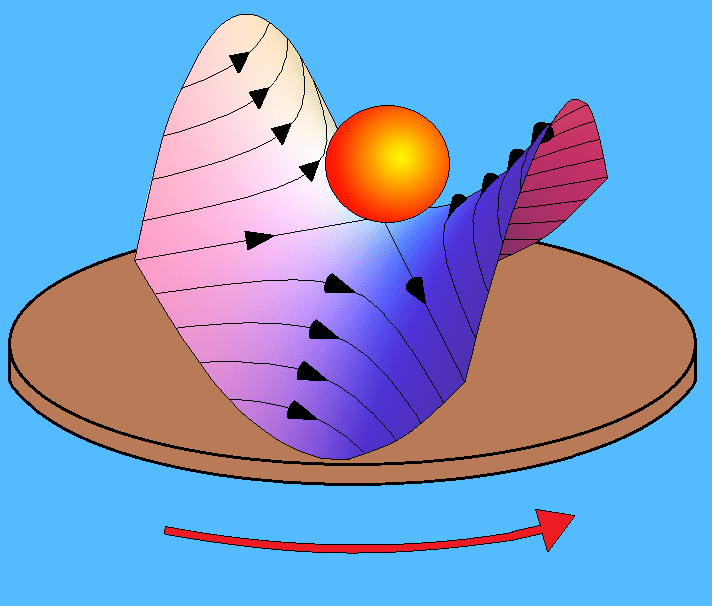
\includegraphics[width=0.48\textwidth]{rotatingSaddle.png}
	\end{center}
	\vspace{-2mm}
	\caption{Mechanical analog of a Paul Trap. Gravitational potential creates a saddle point. The rotation of the potential confines the ball to the center of the well}
	\label{fig:mech}
	\vspace{-3mm}
\end{figure}
%%%%%%%%%%%%%%%%%%%%%%	
%%%%%%%%%%%%%%%%%%%%%%%%%%%%%%%%
%%%%%%%%%%%%%%%%%%%%%%%%%%%%%%%%
Now matching the 0th order terms allows us to solve for A.
\begin{equation}
-A^2=q_xB=-\frac{q_x^2}{2}
\end{equation}
giving
\begin{equation}
A=\frac{q_x}{\sqrt{2}}
\end{equation}
Finally plugging our values for $A$ and $B$ back into equation \ref{eq:mathSol} we find the displacement in the $\hat{e}_x$ direction to be.
\begin{equation}
x=x_0\cos\left(\frac{q_x\tau}{\sqrt{2}}+\theta_0\right)\left(1+\frac{q_x}{2}\cos{2\tau}\right)
\end{equation}
We can see that in the limit of $q_x\ll1$ the motion will behave as a harmonic oscillator confining the electron in the $\hat{e}_x$ and $\hat{e}_y$ directions. Remembering that we defined $q_x\equiv\frac{2eV_0}{\Omega^2Mr_0^2}$, we can see that as long as the wavelength of the driving frequency $\omega$ is large compared to that of the oscillation amplitudes in the electrodes this assumption is valid. And hence the particles are stationary in the trap oscillating at a frequency of 
\begin{equation}
\omega_c = \frac{q_x\Omega}{2\sqrt{2}}=\frac{eV_0}{\sqrt{2}\Omega Mr_0}
\end{equation}
If we now add 2 positively charged end caps the ions are trapped in all 3 spacial dimensions. 
%%%%%%%%%%%%%%%%%%%%%%%%%%%%%%%%
%%%%%%%%%%%%%%%%%%%%%%%%%%%%
\begin{figure}
	\begin{center}
		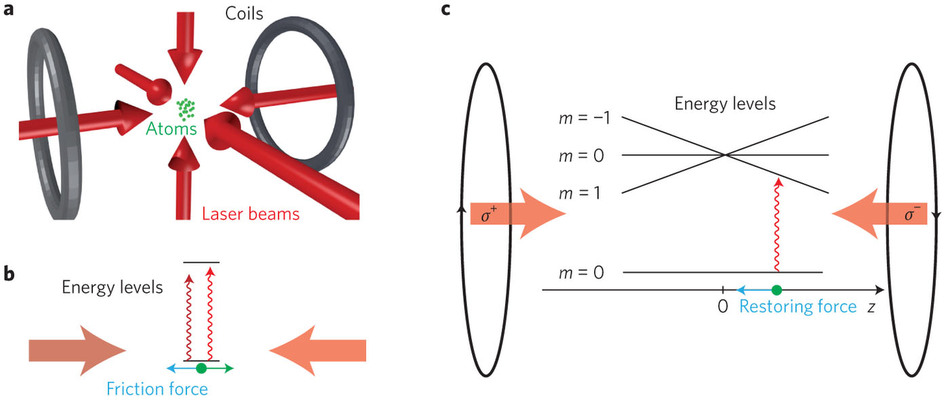
\includegraphics[width=0.48\textwidth]{laserCooling}
	\end{center}
	\vspace{-2mm}
	\caption{a) Six beam laser cooling, lasers create a restoring force known as "optical molasses, which slows atoms localizing them about the center of the beams. b)Beams are slightly tuned to a lower frequency "red tuned" so that only atoms moving toward the laser will absorb the photon slowing it down. This is due to the Doppler effect and it assures that no photon collisions increase the velocity of the particle.\cite{esteve2013cold}}
	\label{fig:laser}
	\vspace{-3mm}
\end{figure}
%%%%%%%%%%%%%%%%%%%%%%	
%%%%%%%%%%%%%%%%%%%%%%%%%%%%%%%%



The fundamental piece of information in a classical computer is called a bit. Similarly the fundamental piece of information in a quantum computer is a qbit. Where the bit is a binary value $0$ or $1$ the quit is derived from a two level quantum system, such as a particle's spin or the hyperfine levels of an atom. While a single qbit exists as a superposition of states i.e.
\begin{equation}
\psi_{qbit}=a\ket{\downarrow}+b\bra{\uparrow}
\end{equation}
it does not by its self carry more information that a single classical bit. It is only when a particle is entangled with other quantum particles that the quantum bits become more efficient than classical bits. Entanglement occurs when a quantum particle or particles interact in a way such that the quantum state of each individual particle can not be described without information from the other entangled particles. It is only when the quantum state of the system as a whole is described that the information about the individual particles can be known. In a quantum calculation the states of the individual qbits are initialized and then XOR operations which are defined to manipulate the overall quantum state are performed. Finally the wavefunction is collapsed and quantum information is turned into classical information.
%%%%%%%%%%%%%%%%%%%%%%%%%%%%%%%%
%%%%%%%%%%%%%%%%%%%%%%%%%%%%
\begin{figure}
	\begin{center}
		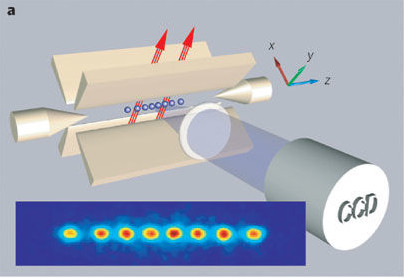
\includegraphics[width=0.48\textwidth]{trappedIons}
	\end{center}
	\vspace{-2mm}
	\caption{Linear Paul trap with individually separated laser cooled ions.Inset is a ccd camera image which shows the separation to be $\approx8\mu m$ \cite{esteve2013cold}}
	\label{fig:sepIons}
	\vspace{-3mm}
\end{figure}
%%%%%%%%%%%%%%%%%%%%%%	
%%%%%%%%%%%%%%%%%%%%%%%%%%%%%%%%

The birth of experimental quantum computing can be traced back to two key papers. The first, by Ignacio Cirac and Peter Zoller describing a physical system which was able to implement quantum algorithms \citealp{cirac1995quantum}. Followed by a paper by David Wineland's group at NIST which showed that it was possible to "flip" a single qbit in such a system \cite{monroe1995demonstration}. To this day of the many methods of creating a quantum computer, currently experiments using trapped ions are the furthest advanced. In these experiments ions are trapped using electromagnetic potentials as described above. Quantum information is transferred through the collective quantized motion of the system of entangled ions. But in order for the individual ions to behave quantum mechanically the ions must be isolated from their environment and the thermal kinetic energy must be much less than the energy put into the system when performing the computations.  In the case of trapped ions the calculations are carried out using. The energy associated with gaining or emitting an electron (known as recoil energy) is on the order of $2\times 10^{-29}J$.
 
From this we can tell that the system must be cooled down to the order of $T\approx1\mu K$ in order to perform accurate quantum calculations.
This cooling is done through laser cooling. Laser cooling uses the momentum of incoming photons to slow down a particle. The lasers are tuned to a slightly lower frequency than the resonant frequency of the particle so that only the particles traveling in the opposite direction to the photon (which are Doppler shifted to a higher frequency) are slowed down due to photon absorption Thus by applying one laser for each spacial direction the particles can be cooled to near absolute zero (Fig. \ref{fig:laser})

Once the ions are effectively cooled the entire ion trap consists of a single quantum register with each trapped ion representing a single qbit In order to perform quantum computations we must be able to initialize the system by manipulating a single photon without affecting the surrounding qbits. This can be done by pumping the relevant ion with a light pulse, exciting it to the desired hyperfine level. This is possible because the individual ions trapped in a Paul trap are separated by $\approx20\mu m$ (Fig.  \ref{fig:sepIons})

While ion traps have been shown to be able to carry out quantum calculations they have a problem with scalability, with some papers limiting their computations to the order of 10s of ions \cite{wineland1998experimental,bartlett2001experimental}. This is due to trapped ion quantum computers being limited to single and multi qbit gates each requiring its own individually controlled and stabalized laser beam. This has lead to some papers working on methods implementing parallel arrays of traps\cite{kielpinski2002architecture} and others working on microwave trapped ion computers \cite{lekitsch2017blueprint}. It is unclear which form the quantum computer will take in the long run but trapped ion quanum computers offer a promising vision into what was once deemed science fiction.

%%%%%%%%%%%%%%%%%%%%%%%%%%%%%%%%%%%%%%%%%%%%%%%
	
\begin{thebibliography}{100}
	
    \bibitem{esteve2013cold} E. J{\'e}r{\^o}me Nature nanotechnology \textbf{8}, 317 (2013)
	\bibitem{blatt2008entangled} R. Blatt and D. Wineland Nature \textbf{453}, 317 (2008)
	\bibitem{cirac1995quantum} I. Cirac and P. Zoller Physical review letters \textbf{74} 4091 (1995)
	\bibitem{monroe1995demonstration} C. Monroe D.M. King, and B.E. Etano, D. J. Wineland Physical review letters \textbf{74} 4714 (1995)
	\bibitem{lekitsch2017blueprint} B. Lekitsch, S. Weidt, A.G. Fowler, K. M{\o}lmer, S.J. Devitt, C.Wunderlich, W.K. Hensinger,Science Advances \textbf{3} 2 (2017)
	\bibitem{kielpinski2002architecture} D. Kielpinski, C. Monroe, D.J. Wineland, Nature \textbf{417} 709 (2002)
	\bibitem{wineland1998experimental} D.Wineland, C. Monroe, W.M. Itano, D. Leibfried, B.E. King, D.M. Meekhof, Journal of Research of NIST \textbf{103}, 259 (1998)
	\bibitem{bartlett2001experimental} S.D.Bartlett, B.C. Sanders, and H de Guise Rinton, Princeton. NJ 344 (2008)
	
	
\end{thebibliography}

\end{document}
%
% ****** End of file apstemplate.tex ******

